\documentclass[letterpaper,12pt]{article}
\usepackage{bookmark}
\usepackage[utf8]{inputenc}
\usepackage[spanish,es-tabla]{babel}
\usepackage{amsfonts}
\usepackage{graphicx}
\usepackage{mathptmx}
\usepackage{float}
\usepackage[T1]{fontenc}
\usepackage[margin=1.3in]{geometry}
\usepackage{amsthm}
\usepackage{marvosym}
\usepackage{bm}

\renewcommand\qedsymbol{\Squarepipe}

\theoremstyle{definition}
\newtheorem{definition}{Definición}[section]
\newtheorem*{thm}{Teorema}


\setlength\parindent{0pt}

\newcounter{paragraphnumber}
\newcommand{\para}{%
  \vspace{10pt}\noindent{\bfseries\refstepcounter{paragraphnumber}\theparagraphnumber.\quad}%
}

%\setsecheadstyle{\large\bfseries}
%\setsubsecheadstyle{\bfseries}

\setlength\parindent{0pt}

\pagenumbering{gobble}

%\usepackage[margin=1in]{geometry}

\usepackage{enumitem}
\setlist{nosep}

\usepackage{xcolor}

\usepackage{hyperref}
\hypersetup{
  colorlinks,
  linkcolor={red!50!black},
  citecolor={blue!50!black},
  urlcolor={green!50!black}
}

\usepackage{amssymb}
\usepackage{amsmath}

\begin{document}

\begin{center}
  {\large Cómputo Evolutivo}\\
  \vspace{0.2cm}
  {\large\bfseries Tarea 1}\\
  \vspace{0.2cm}
  {\large PCIC - UNAM}\\
  \vspace{0.5cm}
  {\itshape 19 de febrero de 2020}\\
  \vspace{0.5cm}
  Diego de Jesús Isla López\\
  (\href{mailto:dislalopez@gmail.com}{\itshape dislalopez@gmail.com})\\
  (\href{mailto:diego.isla@comunidad.unam.mx}{\itshape diego.isla@comunidad.unam.mx})\\
\end{center}



\section*{Definición del problema}

Implementar el algoritmo genético en su versión con codificación binaria y con los siguientes operadores:\\

\begin{itemize}
  \item Selección:
    \begin{itemize}
      \item Método de ruleta
      \item Torneo binario
      \item Selección estocástica universal
      \item Método de Vasconcelos
    \end{itemize}
  \item Cruza: aleatoria en un punto con tasa de $0.9$
  \item Mutación: aleatoria con tasa de \(\frac{0.1}{L}\) donde \(L\) es la longitud del individuo
  \item Elitismo
\end{itemize}

\medskip

Además, deben configurarse los siguientes parámetros:\\

\begin{itemize}
  \item Población: $100$ individuos
  \item Número de generaciones: $500$
\end{itemize}

\section*{Función de aptitud}

Para las funciones Rastrigin y Himmelblau se usó la siguiente función de aptitud:

\begin{equation*}
  fit = \frac{1}{f(x)}
\end{equation*}

donde \(f(x))\) es el valor de la función objetivo encontrado por el algoritmo.
Para el caso de la función Eggholder, se optó por solo aplicar \(fit = -f(x)\).


\section*{Resultados}

\subsection*{Algoritmo GA con selección por ruleta}

En la figura \ref{fig:rast_basic} se muestra el desempeño del algoritmo con la función Rastrigin. Como se observa, la aptitud se mantiene relativamente estática durante gran parte de la ejecución para después dar un salto hacia soluciones con un valor muy alto de aptitud. En la gráfica de valores de función objetivo, es posible ver cómo éstos decrecen precipitadamente para después mantenerse estables, lo cual sucede en etapas tempranas de la ejecución.\\

Para el caso de la función Himmelblau (figura \ref{fig:egg_basic}), es posible ver en la gráfica de valores de aptitud que el desempeño tiene un crecimiento gradual con algunos picos antes de quedar estable. En la gráfica de valores objetivo, es posible apreciar un descenso uniforme.\\

Sin embargo, para la función Eggholder (figura \ref{fig:egg_basic}) notamos que existe un comportamiento irregular. Existen muchos picos y la tendencia se aprecia hacia la baja en la gráfica de aptitud mientras que en la de función objetivo es a la alza, lo cual es un comportamiento no deseado. Sin embargo, este comportamiento mejora con la aplicación de elitismo y de otros métodos de selección.

\begin{figure}[H]
  \minipage{0.49\textwidth}
    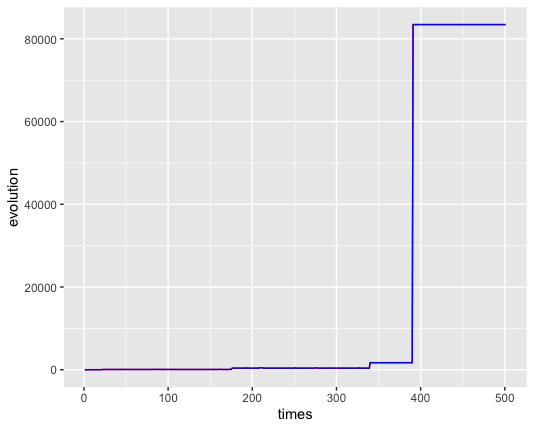
\includegraphics[width=\linewidth]{rast_basic_fitness}
    %\caption{Valores de aptitud}
  \endminipage\hfill
  \minipage{0.49\textwidth}
    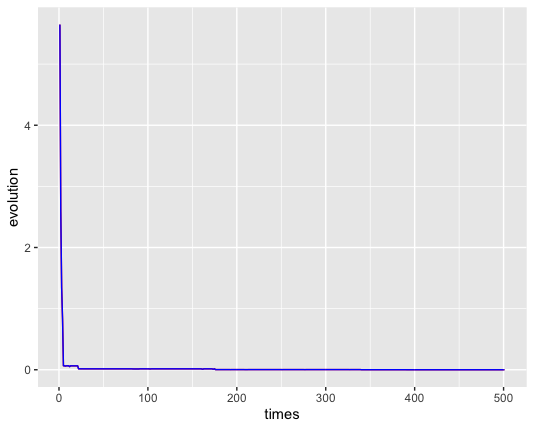
\includegraphics[width=\linewidth]{rast_basic_eval}
    %\caption{Valores de función objetivo}
  \endminipage\hfill
  \caption{Función Rastrigin con GA básico y selección por ruleta}
  \label{fig:rast_basic}
\end{figure}

\begin{figure}[H]
  \minipage{0.49\textwidth}
    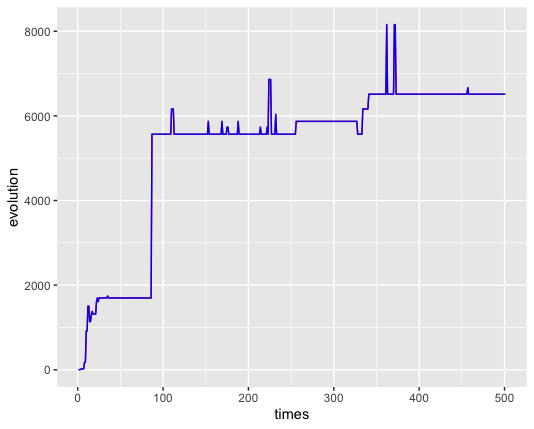
\includegraphics[width=\linewidth]{himm_basic_fitness}
    %\caption{Valores de aptitud}
  \endminipage\hfill
  \minipage{0.49\textwidth}
    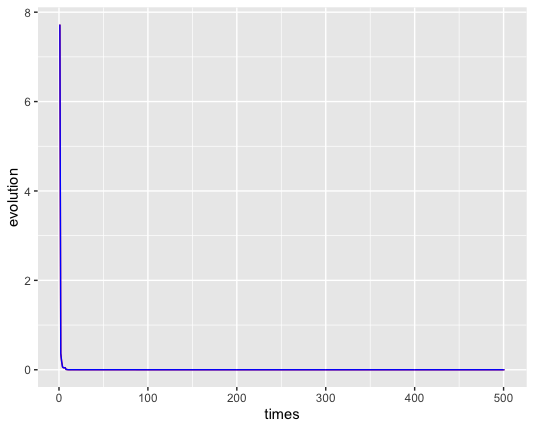
\includegraphics[width=\linewidth]{himm_basic_eval}
    %\caption{Valores de función objetivo}
  \endminipage\hfill
  \caption{Función Himmelblau con GA básico y selección por ruleta}
  \label{fig:him_basic}
\end{figure}

\begin{figure}[H]
  \minipage{0.49\textwidth}
    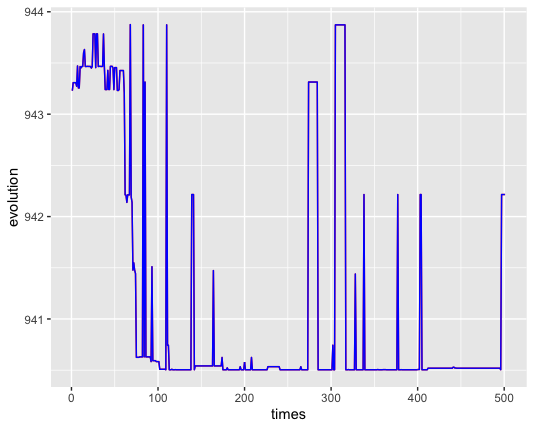
\includegraphics[width=\linewidth]{egg_basic_fitness}
    %\caption{Valores de aptitud}
  \endminipage\hfill
  \minipage{0.49\textwidth}
    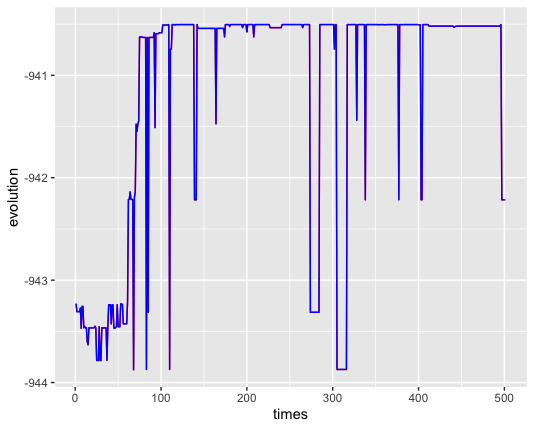
\includegraphics[width=\linewidth]{egg_basic_eval}
    %\caption{Valores de función objetivo}
  \endminipage\hfill
  \caption{Función Eggholder con GA básico y selección por ruleta}
  \label{fig:egg_basic}
\end{figure}


\subsection*{Algoritmo GA con elitismo}

El operador de elitismo utilizado para las pruebas consiste en ordenar los individuos actuales en función de su valor de aptitud y tomar a los diez mejores, los cuales se conservarán. La nueva población consistirá de estos individuos y el restante de los hijos generados durante la cruza. \\

\textbf{Selección por torneo}\\

La modalidad de torneo elegida fue binaria (torneo entre pares de individuos). \\


En el caso de la función Rastrigin (figura \ref{fig:rast_tour}) se puede apreciar un comportamiento de incremento constante en los valores de aptitud para después estabilizarse, lo cual sucede en etapas tempranas. Análogamente, el descenso en los valores de función objetivo es constante.\\

Para la función Himmelblau (figura \ref{fig:him_tour}), es posible ver que el comportamiento de los valores de aptitud tiene una tendencia más uniforme que la vista anteriormente. La evolución de la aptitud mejora gradualmente durante las primeras generaciones para después tener un salto de mejora alrededor de las 150 generaciones y estabilizarse.\\

Al evaluar la función Eggholder, es evidente la mejora en el desempeño con respecto al algoritmo base y la selección con ruleta. El comportamiento es mucho más estable y gradual, sin perturbaciones mayores y con una convergencia que sucede alrededor de la mitad del número de generaciones.


\begin{figure}[H]
  \minipage{0.49\textwidth}
    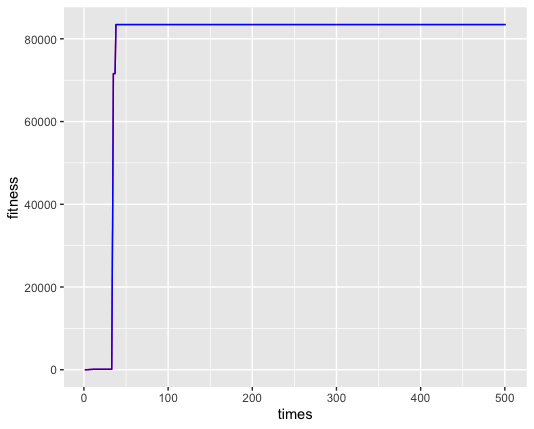
\includegraphics[width=\linewidth]{rast_tour_fitness}
    %\caption{Valores de aptitud}
  \endminipage\hfill
  \minipage{0.49\textwidth}
    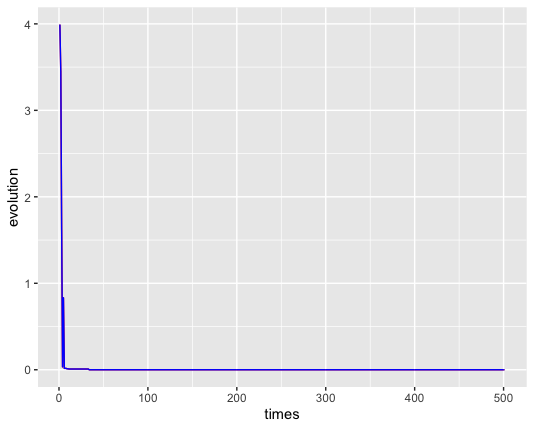
\includegraphics[width=\linewidth]{rast_tour_eval}
    %\caption{Valores de función objetivo}
  \endminipage\hfill
  \caption{Función Rastrigin selección por torneo}
  \label{fig:rast_tour}
\end{figure}

\begin{figure}[H]
  \minipage{0.49\textwidth}
    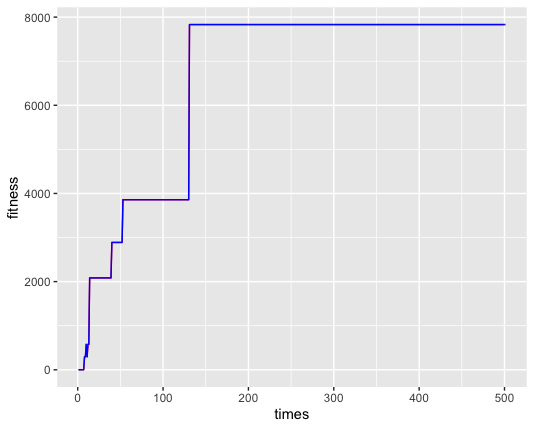
\includegraphics[width=\linewidth]{him_tour_fitness}
    %\caption{Valores de aptitud}
  \endminipage\hfill
  \minipage{0.49\textwidth}
    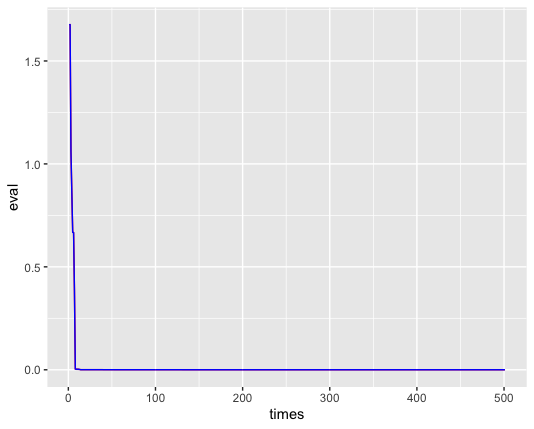
\includegraphics[width=\linewidth]{him_tour_eval}
    %\caption{Valores de función objetivo}
  \endminipage\hfill
  \caption{Función Himmelblau selección por torneo}
  \label{fig:him_tour}
\end{figure}

\begin{figure}[H]
  \minipage{0.49\textwidth}
    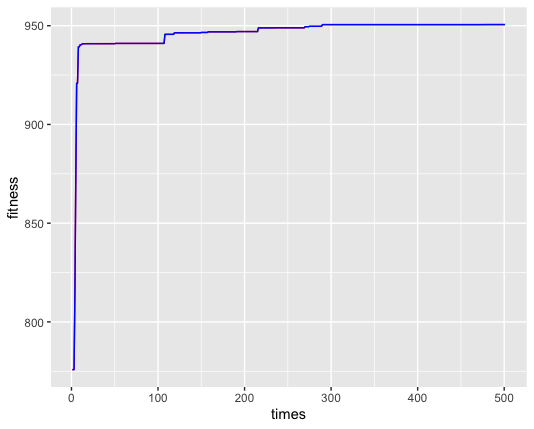
\includegraphics[width=\linewidth]{egg_tour_fitness}
    %\caption{Valores de aptitud}
  \endminipage\hfill
  \minipage{0.49\textwidth}
    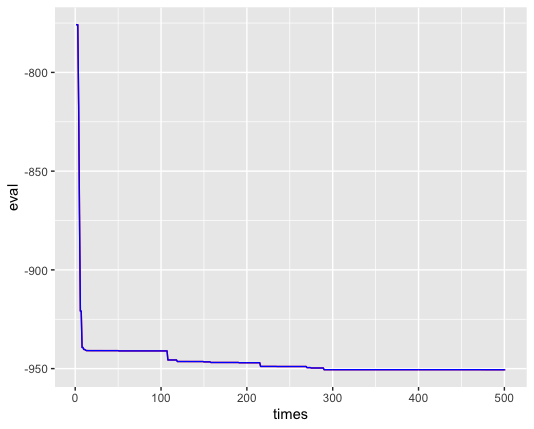
\includegraphics[width=\linewidth]{egg_tour_eval}
    %\caption{Valores de función objetivo}
  \endminipage\hfill
  \caption{Función Eggholder selección por torneo}
  \label{fig:egg_tour}
\end{figure}


\textbf{Selección estocástica universal}\\

Con este método es visible que para los tres problemas, la evolución del valor de la función objetivo es ligeramente más gradual que en los otros métodos. Es visible la tendencia a mejorar la aptitud. En la función Himmelblau (figura \ref{fig:him_sus}) se puede apreciar un incremento escalonado del valor de la aptitud, con pequeñas mejoras hasta llegar a las 350 generaciones donde se da una mejora importante. Para el caso de la función Eggholder (figura \ref{fig:egg_sus}), es posible apreciar que en las últimas generaciones es capaz de tener pequeñas mejoras.

\begin{figure}[H]
  \minipage{0.49\textwidth}
    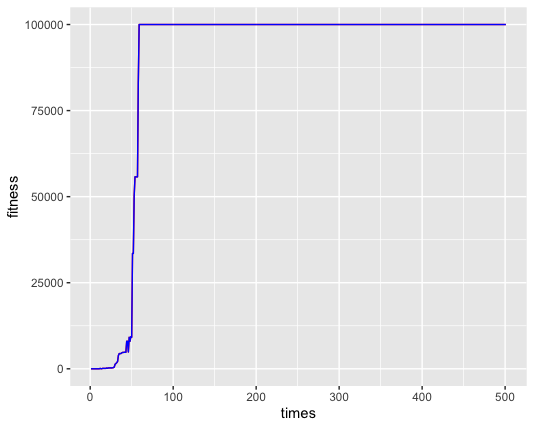
\includegraphics[width=\linewidth]{rast_elite_sus_fitness_new}
    %\caption{Valores de aptitud}
  \endminipage\hfill
  \minipage{0.49\textwidth}
    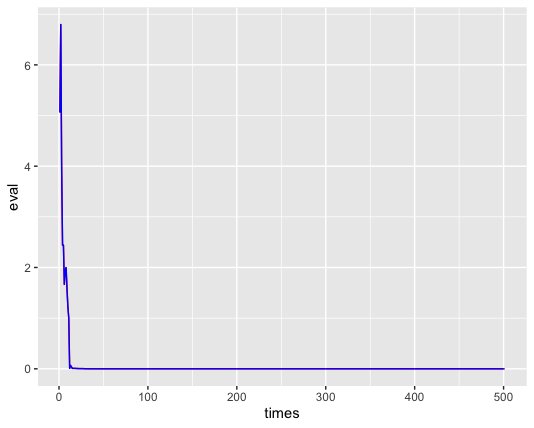
\includegraphics[width=\linewidth]{rast_elite_sus_eval_new}
    %\caption{Valores de función objetivo}
  \endminipage\hfill
  \caption{Función Rastrigin selección por SUS}
  \label{fig:rast_sus}
\end{figure}

\begin{figure}[H]
  \minipage{0.49\textwidth}
    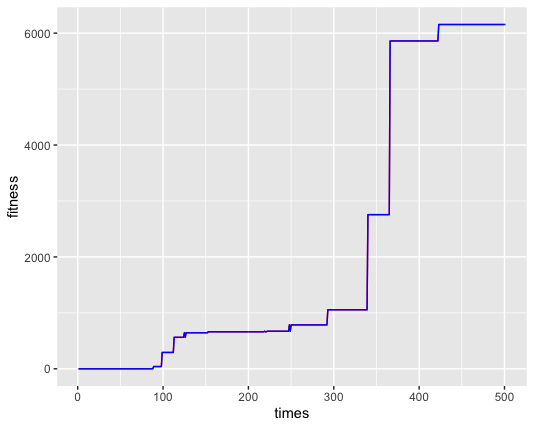
\includegraphics[width=\linewidth]{him_elite_sus_fitness_new}
    %\caption{Valores de aptitud}
  \endminipage\hfill
  \minipage{0.49\textwidth}
    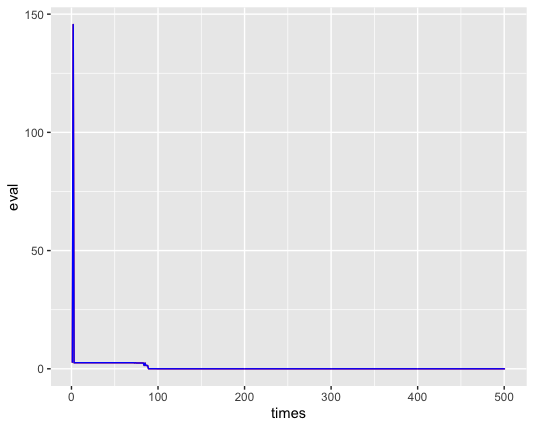
\includegraphics[width=\linewidth]{him_elite_sus_eval_new}
    %\caption{Valores de función objetivo}
  \endminipage\hfill
  \caption{Función Himmelblau selección por SUS}
  \label{fig:him_sus}
\end{figure}

\begin{figure}[h!]
  \minipage{0.49\textwidth}
    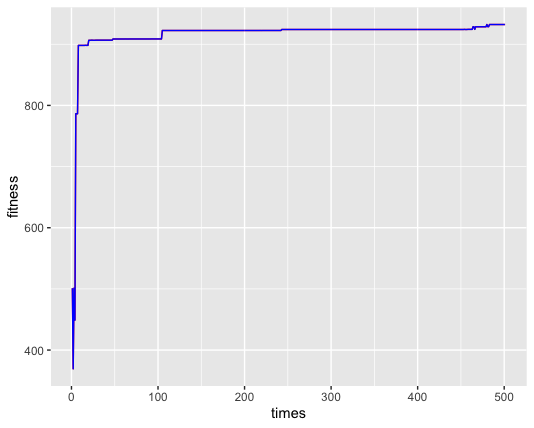
\includegraphics[width=\linewidth]{egg_elite_sus_fitness_new}
    %\caption{Valores de aptitud}
  \endminipage\hfill
  \minipage{0.49\textwidth}
    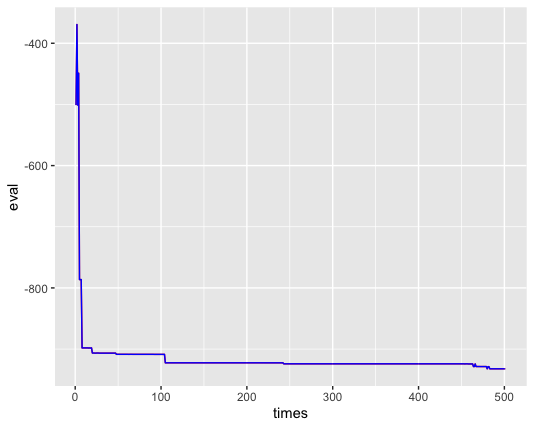
\includegraphics[width=\linewidth]{egg_elite_sus_eval_new}
    %\caption{Valores de función objetivo}
  \endminipage\hfill
  \caption{Función Eggholder selección por SUS}
  \label{fig:egg_sus}
\end{figure}

\textbf{Método de Vasconcelos}\\

Para este método de selección, es de hacer notar el comportamiento presentado al evaluar la función Himmelblau (figura \ref{fig:him_vas}), donde se tiene una evolución muy lenta para después converger de manera muy rápida en las últimas generaciones. Sin embargo, la disminución en el valor de la función objetivo es uniforme.\\

Tanto para la función Rastrigin como para la función Eggholder (figuras \ref{fig:rast_vas} y \ref{fig:egg_vas}) el comportamiento es muy uniforme, presentándose perturbaciones menores, en particular para la función Rastrigin. Ambas convergen alrededor de la marca de 100 generaciones.


\begin{figure}[H]
  \minipage{0.49\textwidth}
    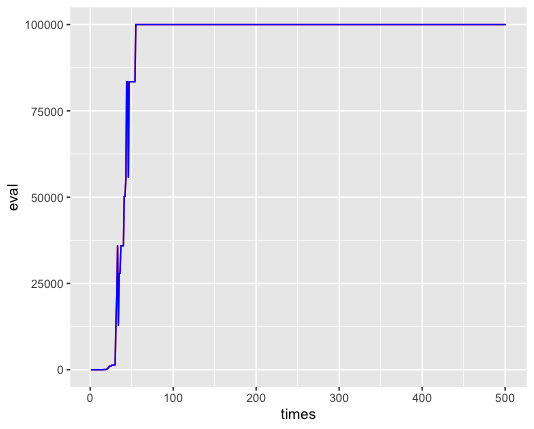
\includegraphics[width=\linewidth]{rast_vas_fitness}
    %\caption{Valores de aptitud}
  \endminipage\hfill
  \minipage{0.49\textwidth}
    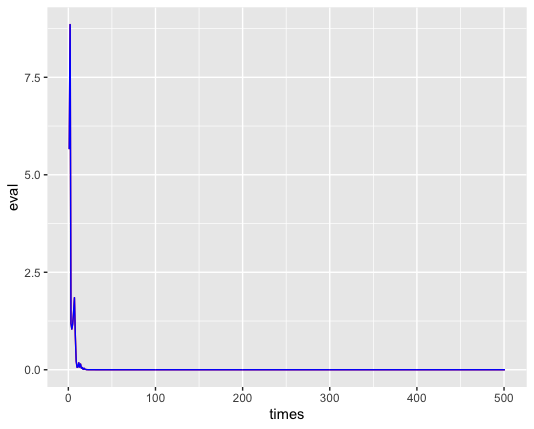
\includegraphics[width=\linewidth]{rast_vas_eval}
    %\caption{Valores de función objetivo}
  \endminipage\hfill
  \caption{Función Rastrigin selección por Vasconcelos}
  \label{fig:rast_vas}
\end{figure}

\begin{figure}[H]
  \minipage{0.49\textwidth}
    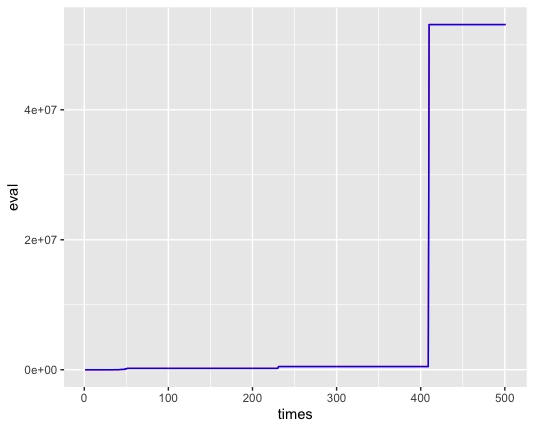
\includegraphics[width=\linewidth]{him_vas_fitness}
    %\caption{Valores de aptitud}
  \endminipage\hfill
  \minipage{0.49\textwidth}
    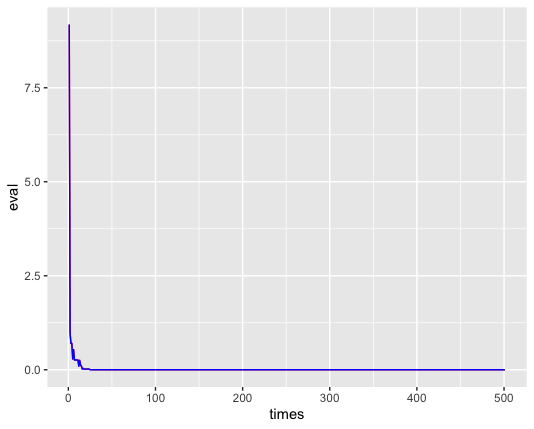
\includegraphics[width=\linewidth]{him_vas_eval}
    %\caption{Valores de función objetivo}
  \endminipage\hfill
  \caption{Función Himmelblau selección por Vasconcelos}
  \label{fig:him_vas}
\end{figure}

\begin{figure}[H]
  \minipage{0.49\textwidth}
    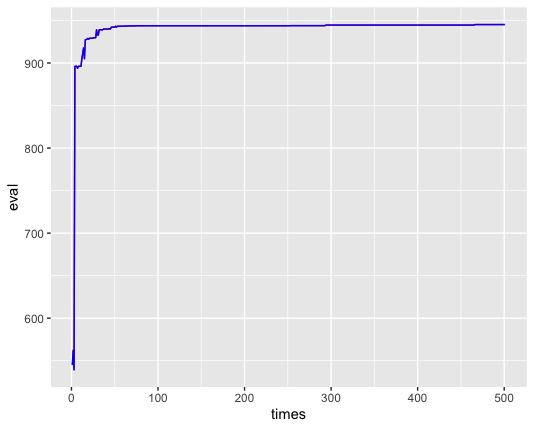
\includegraphics[width=\linewidth]{egg_vas_fitness}
    %\caption{Valores de aptitud}
  \endminipage\hfill
  \minipage{0.49\textwidth}
    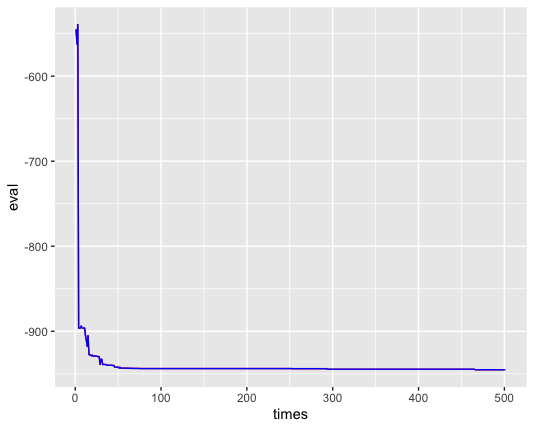
\includegraphics[width=\linewidth]{egg_vas_eval}
    %\caption{Valores de función objetivo}
  \endminipage\hfill
  \caption{Función Eggholder selección por Vasconcelos}
  \label{fig:egg_vas}
\end{figure}

\section*{Conclusiones}

Se observa que la diferencia de desempeño entre el algoritmo base y después de aplicar elitismo es notoria. Además, es posible observar la influencia que tienen los diferentes métodos de selección en la convergencia hacia los valores óptimos. Todos los métodos tiene un comportamiento estable, sin embargo es evidente que la selección por torneo tiene un comportamiendo más gradual y logra encontrar mejores soluciones. Se puede apreciar también que el método SUS es capaz de hacer mejoras en las últimas generaciones, como fue posible ver para el caso de la función Eggholder.

\end{document}